\begin{frame}{TCP state machine}
\begin{tikzpicture}
\node (state) {
    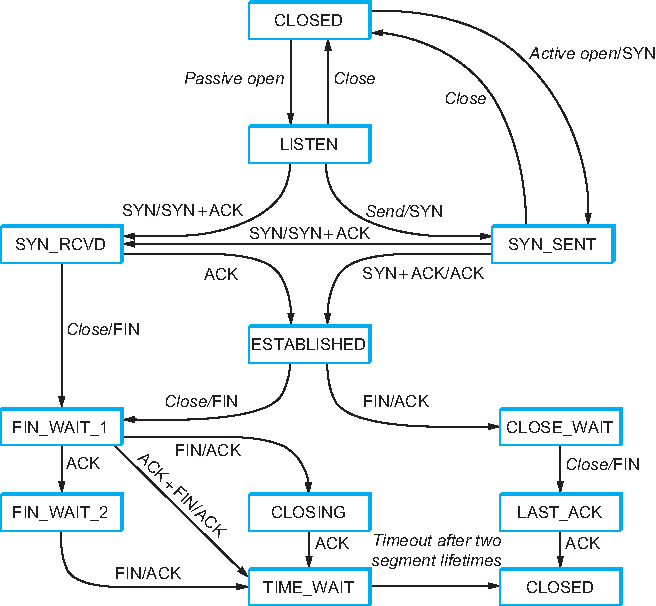
\includegraphics[height=0.8\textheight]{../sockets/sysapproach-tcp-state-fig}
};
\node[anchor=north west, align=left] at (state.north east) {
   notation: event/action  \\
   ~ \\
   not shown explicitly: timeout/resend
};
\end{tikzpicture}
\end{frame}


\begin{frame}{connection close}
    \begin{itemize}
    \item FIN (I want to close) + ACK (confirm close)
    \vspace{.5cm}
    \item ACK side needs to wait just in case FIN resent
        \begin{itemize}
        \item keep port number from being reused
        \item TIME\_WAIT state
        \end{itemize}
    \end{itemize}
\end{frame}

\begin{frame}{RST}
    \begin{itemize}
    \item RST (reset) flag often used to respond to unexpected packets
    \item example: data packet for never-established connection
    \end{itemize}
\end{frame}
